\documentclass[11pt]{article}
\usepackage[margin=1in]{geometry} 
\usepackage{amsmath,amsthm,amssymb}
\usepackage{hyperref}
\usepackage{caption}
\usepackage{subcaption}
\usepackage{graphicx}
\usepackage{authblk}
\usepackage{enumitem}
\hypersetup{
    colorlinks=true,
    linkcolor=cyan,
    filecolor=magenta,      
    urlcolor=cyan,
}

\renewcommand\Authfont{\fontsize{10}{14.4}\selectfont}
\renewcommand\Affilfont{\fontsize{8}{10.8}\itshape}
 
\urlstyle{same}
\setcounter{secnumdepth}{5}
%
\begin{document}
% title
\title{Fall 2019 Capstone Project Progress Report 1 \\
    \small \href{https://github.com/rmahajan14/capstone_didi}{Github}}

%\thanks{Supported by Mult x.} % if we want to thank someone/org.
%
% authors

\author[1]{Ridhi Mahajan}
\author[2]{Akshat Mittal}
\author[3]{Nima Chitsazan}
\author[4]{Foad Khoshouei}
\author[5]{Ashwin Jayaraman}
\author[6]{Vineet Goyal\thanks{vgoyal@ieor.columbia.edu}} 
\author[7]{Zhiwei (Tony) Qin\thanks{qinzhiwei@didiglobal.com}}

\affil[1,2,3,4,5]{Data Science Institute, Columbia University, New York, NY, USA}
\affil[6]{IEOR, Columbia University University, New York, NY, USA}
\affil[7]{DiDi Labs / AI Labs, Mountain View, CA, USA}


% \author{Ridhi Mahajan, Akshat Mittal, Nima Chitsazan, Foad Khoshouei, Ashwin Jayaraman}

% \author{Ridhi Mahajan\\\affil{rm3601}\and Akshat Mittal\\\affil{am5022} \and Nima Chitsazan\\\affil{nc2806}\and Foad Khoshouei\\\affil{fk2377}\and Ashwin Jayaraman\\\affil{aj2844}}

\maketitle              % typeset the header of the contribution
%

%
%
%
\section{Project Introduction}
The aim of the project is to identify the metrics which allow a driver to be successful on the Didi platform. The ride hailing platform allows drivers the flexibility to choose when they can get online and how long they stay online. It also tells the drivers where to go when they are not assigned an order, typically based on their habits and preferences. 
\\\\
But it can be seen that despite similar work hours and period of activity, some drivers are able to perform better than their coworkers.  This could be seen by the difference in their in-service hours. Even if different drivers are online for the same amount of time, their in-service time, or total time of rides, is often different. 
\\\\
Through this project, we try to understand the relationship and differences between the drivers' in-service hours and their work patterns. Any insights obtained from this task could be extremely useful to identify best practices that could be shared with the drivers and improve their efficiency on the platform.

\section{Literature Review}
The online ride hailing companies are growing at a rapid rate and innovation is a key driver of their business model. Since the GPS trajectories are increasingly more available, machine learning and data analysis can be used to uncover drivers' habits and strategies and their effectiveness. Liu et al. (2010) used taxi GPS data to analyze travel demand distribution, DBSCAN algorithm to cluster pick-up and drop-off locations, and used spatial interaction models to study and compare the searching behavior of the cab drivers in Harbin City, China. In their study, the trips for the taxis were classified into two groups based on their activity: (1) pick-up a passenger from the origin and drop-off at destination (we call this active time in this report) and (2) roam around the city to find the next passenger (we call this inactive time in this report). These are analogous to online ride hailing platforms as well since the driver has to wait for the app to assign the next order to pick-up a passenger. However the behavior of the drivers in a traditional taxi system is different from the drivers on an online ride hailing systems. The traditional taxi drivers have to search for their next passenger while on the online ride hailing platforms a passenger is assigned to the driver and the drivers have to re-position themselves in a way that the platform can match them with a passenger. 

Lie et al. (2011) concluded that it is more efficient to hunt for passengers compared to waiting by comparing taxi drivers' behavior and profitability. The pattern and behavior of the more efficient drivers can provide an understanding of their strategy and help to provide recommendations to other drivers as well. Vacant cars roaming on the streets generate additional traffic, pollution and are less efficient. The dispatching system for online ride haling platforms must make decisions both for assigning drivers to passengers and also re-positioning drivers who have no nearby orders.   Shou et al. (2019) used a Markov Decision Process to model optimal sequential decisions in passenger seeking. In their study, the reward function was estimated using an inverse reinforcement learning technique trained on 3-day trajectories of GPS data from DiDi. Holler et al. (2018) proposed a global state representation along with a neural network that can produce action-values (Q-values) for a reinforcement learning problem. This problem has been studied extensively , see [7,8].


\section{Initial Data Exploration/Visualization}
\subsection{Dataset Description}
The dataset used is the GAIA Open Dataset which is available through \href{https://outreach.didichuxing.com/research/opendata/en/}{DiDi}.  We have access to the following tables for the month of November, 2016 : 
\begin{enumerate}
\item $GPS$ - This allows us to determine the trajectory for every ride by the
driver.
 \item $Orders$ - This consists of the statistics for a particular order.
    \begin{table}[h!]
        \centering
         \begin{tabular}{||c c c c||} 
         \hline
         Field & Type & Sample & Comment \\ [0.5ex] 
         \hline\hline
         Driver ID & String & glox.jrrlltBMvCh8nxqktdr2dtopmlH & Anonymized \\ 
         \hline
         Order ID & String & jkkt8kxniovIFuns9qrrlvst@iqnpkwz & Anonymized \\
         \hline
         Time Stamp & String & 1501584540 & Unix timestamp, in seconds \\
         \hline
         Longitude & String & 104.04392 & GCJ-02 Coordinate System \\
         \hline
         Latitude & String & 104.04392 & GCJ-02 Coordinate System \\ [1ex] 
         \hline
        \end{tabular}
        \caption{GPS Data}
        \label{table:1}
\end{table}
    \begin{table}[h!]
        \centering
         \begin{tabular}{||c c c c||} 
         \hline
         Field & Type & Sample & Comment \\ [0.5ex] 
         \hline\hline
         Order ID & String & mjiwdgkqmonDFvCk3ntBpron5mwfrqvI & Anonymized \\
         \hline
         Ride Start Time & String & 1501584540 & Unix timestamp, in seconds \\
         \hline
         Ride Stop Time & String & 1501582195 & Unix timestamp, in seconds \\
         \hline
         Pick-up Longitude & String & 104.11225 & GCJ-02 Coordinate System \\
         \hline
         Pick-up Latitude & String & 30.66703 & GCJ-02 Coordinate System \\ 
         \hline
         Drop-off Longitude & String & 104.07403 & GCJ-02 Coordinate System \\
         \hline
         Drop-off Latitude & String & 30.6863 & GCJ-02 Coordinate System \\ [1ex] 
         \hline

        \end{tabular}
        \caption{Orders Data}
        \label{table:2}
\end{table}
\end{enumerate}
\\\\
The GPS table consists of the following columns: 
\begin{enumerate}
    \item $driver\_id$ - The unique driver id for the driver. This is encrypted, and changes each day.
    \item $order\_id$ - The unique id used to determine the ride. The superset of these ids covers all the rides that a driver takes on the platform.
    \item $timestamp$ - The timestamp when the snapshot of the GPS coordinates is stored.
    \item $latitude$ - The latitude of the driver at the current timestamp.
    \item $longitude$ - The longitude of the driver at the current timestamp.
\end{enumerate}
\\\\
The Orders table consists of the following columns: 
\begin{enumerate}
    \item $order\_id$ - The unique id used to determine the ride.
    \item $ride\_start\_timestamp$ - The starting time of the ride.
    \item $ride\_stop\_timestamp$ - The ending time of the ride.
    \item $pickup\_longitude$ - The longitude of the place where the driver picked up the customer.
    \item $pickup\_latitude$ - The latitude of the place where the driver picked up the customer.
    \item $\mathit{dropoff}\_longitude$ - The longitude of the place where the driver dropped off the customer.
    \item $\mathit{dropoff}\_latitude$ - The latitude of the place where the driver dropped off the customer. 
    
\end{enumerate}

\subsection{Data Challenges}
The following are some of the issues with the data provided:

\begin{itemize}
    \item There is no overlap between the $driver\_ids$ on any 2 days. This is because DiDi assigns a new encrypted $driver\_id$ to a driver each day. So, even if a driver has driven for multiple days, we do not have information to link the same driver across days. This limits the time series data available for each driver (1 day instead of 30 days).
    \item Some ride times are unusually long. Given that even going from one extreme end of the city to another would take 2 hours and 45 minutes, all rides with ride times greater than 3 hours (0.006\% of the data) are treated as bad data points, and hence, removed.
    \item The data has pooled rides without any explicit mention of it. This is a positive thing, as it gives us additional features to incorporate into our model.
    \item Idle time is not given in the data. Further, GPS coordinates for when the driver is not on a ride are not available. So there is no way of knowing where the driver spent his/her idle time.
    

\end{itemize}




\subsection{Data Visualization}
The first phase was exploratory data analysis, and visualizing the data before starting data modelling. We made a scatter plot for the in service time of a driver and their active time on the system. The naive algorithm to calculate the activity time for day $i$ was  
\\
\begin{equation}
\label{Naive_Logic}
active\_time_i = max(ride\_stop\_time_i) -\ min(ride\_start\_time_i) 
\end{equation}

One issue in this logic is that there are drivers with a really high active time. This can be seen in Figure \ref{fig:three graphs}. Hence, we update the logic to incorporate the period of inactivity between rides. The inactive or idle time for a ride $j$ is calculated by taking into account the difference between the start of the next ride $j+1$ and the end of the current ride $j$. We then take a threshold of $60$ minutes where a driver is considered inactive if the difference is larger than this threshold. Hence, the original equation is updated as follows:
% \begin{equation*}
%     diff\_ride_j = ride\_start\_time_{j+1}) - ride\_stop\_time_j
% \end{equation*}

% \begin{equation*}
%     in\_active\_time_i = \sum_{all\, rides\, j} min(diff\_ride_j, 60)
% \end{equation*}

% \begin{equation*}
%     active\_time_i = max(ride\_stop\_time_i) - min(ride\_start\_time_i)  - in\_active\_time_i
% \end{equation*}

% \begin{align*}
%     active\_time_i =& max(ride\_stop\_time_i) - min(ride\_start\_time_i)  - in\_active\_time_i \\
%     in\_active\_time_i =& \sum_{all\, rides\, j} min(diff\_ride_j, 60) \\
%     diff\_ride_j =& ride\_start\_time_{j+1} - ride\_stop\_time_j
% \end{align*}


\begin{equation*}
    \mathit{diff}\_ride_j = ride\_start\_time_{j+1} -\ ride\_stop\_time_j
\end{equation*}

\begin{equation*}
    inactive\_time_i = \sum_{all\, rides\, j} min(\mathit{diff}\_ride_j,\ 60)
\end{equation*}

\begin{equation}
\label{No_Threshold}
    active\_time_i = max(ride\_stop\_time_i) -\ min(ride\_start\_time_i)  -\ inactive\_time_i
\end{equation}



We then make this threshold a hyper-parameter itself, instead of hard-coding it. Hence, our final logic is to create a threshold $t$ (currently set to $60$ minutes) where a driver is active for a threshold period after the end of a ride $j$ and active again for the same threshold before the start of the ride $j+1$. We plan to learn this parameter using the distribution of rides, and time between the rides.


\begin{equation*}
    \mathit{diff}\_ride_j = ride\_start\_time_{j+1} -\ ride\_stop\_time_j
\end{equation*}

\begin{equation*}
    inactive\_time_i = \sum_{all\, rides\, j} max(\mathit{diff}\_ride_j - 2t,\ 0) 
\end{equation*}

\begin{equation}
\label{with_threshold}
    active\_time_i = max(ride\_stop\_time_i) -\ min(ride\_start\_time_i)  -\ inactive\_time_i
\end{equation}



\begin{figure}
     \centering
     \begin{subfigure}[b]{0.48\textwidth}
         \centering
         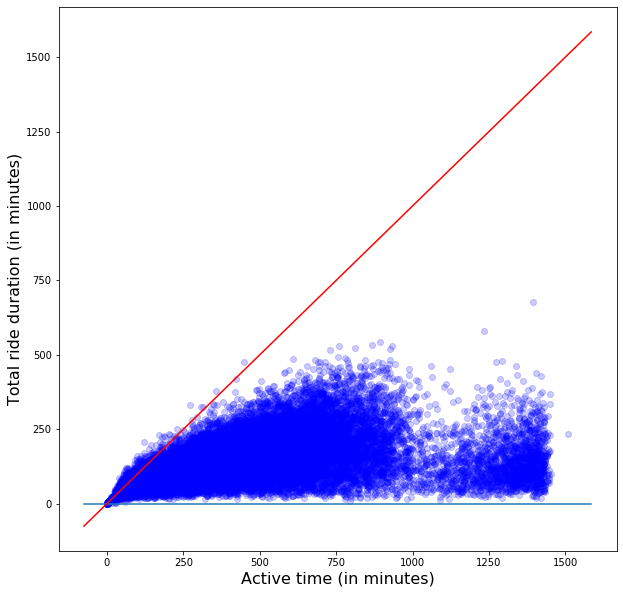
\includegraphics[width=\textwidth]{imgres/original_scatter.png}
         \caption{}
         \label{fig:Active_Time}
     \end{subfigure}
     \hfill
     \begin{subfigure}[b]{0.48\textwidth}
         \centering
         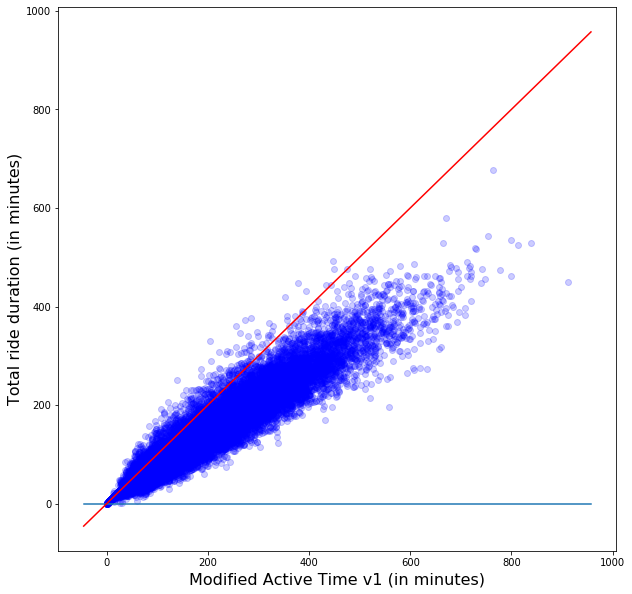
\includegraphics[width=\textwidth]{imgres/mod1_scatter.png}
         \caption{}
         \label{fig:No_threshold_plot}
     \end{subfigure}
     \hfill
     \begin{subfigure}[b]{0.48\textwidth}
         \centering
         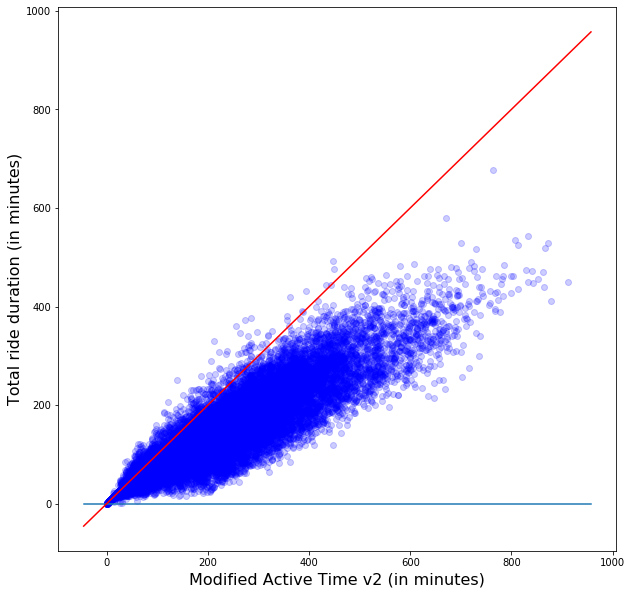
\includegraphics[width=\textwidth]{imgres/mod2_scatter.png}
         \caption{}
         \label{fig:With_threshold_plot}
     \end{subfigure}
        \caption{The plot of the active time with in service hours for November 1st 2016. $(a)$ denotes the naive logic denoted by \ref{Naive_Logic}. $(b)$ denotes the logic where inactivity above an hour was ignored denoted by \ref{No_Threshold}. $(c)$ denotes the logic with a determined threshold denoted by \ref{with_threshold} }
        \label{fig:three graphs}
\end{figure}
\newline

To get an idea of how the pickup locations look at certain snapshots of time on Chengdu City's map, we plot the heatmap of pickup coordinates and drop-off coordinates. This is done to demarcate the residential and industrial areas in Chengdu for 9 A.M. in the morning and 6 P.M. in the evening. The plots shown in Figures \ref{fig:heatmaps9am} and \ref{fig:heatmaps6pm} suggest that there is no clear distinction between where people live and go to work. However, the 9 A.M. drop-off coordinates plot mildly suggests that people tend to end their rides more towards the center of the city as compared to the pickups.

\begin{figure}
    \centering
    \begin{minipage}{0.45\textwidth}
        \centering
        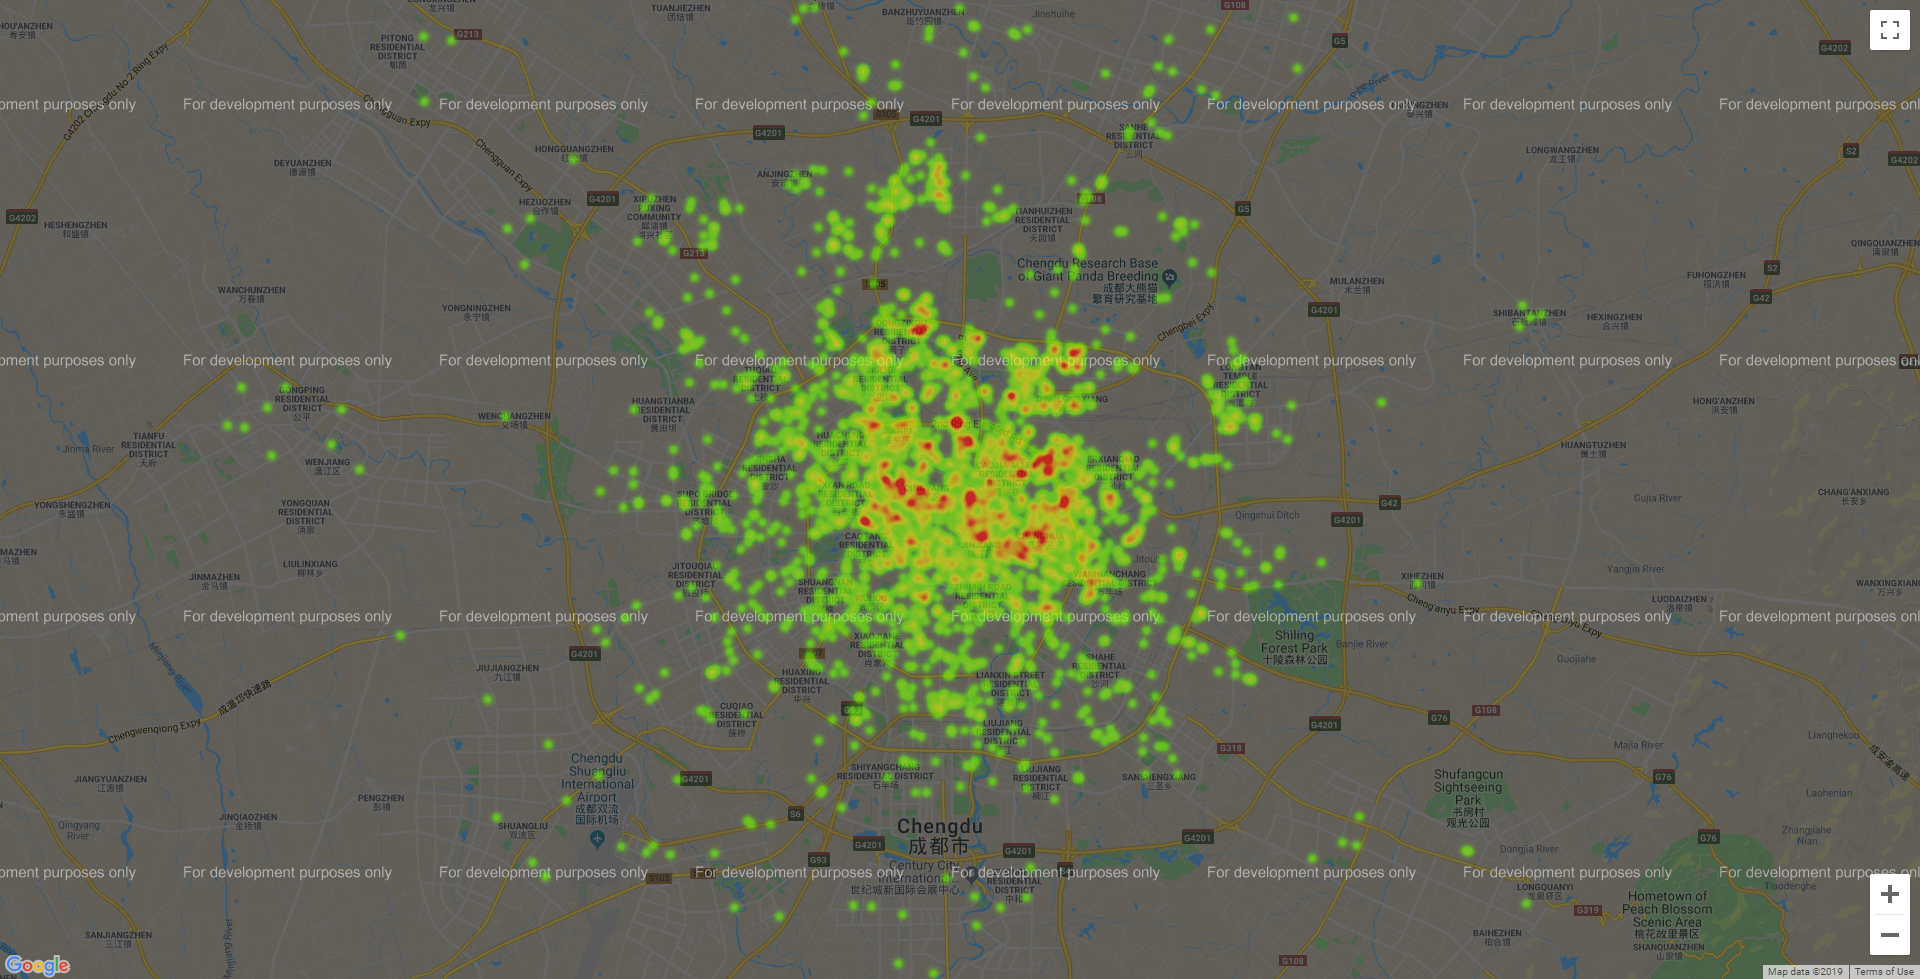
\includegraphics[width=0.9\textwidth]{imgres/9AM_Pickup.PNG} % first figure itself
    \end{minipage}\hfill
    \begin{minipage}{0.45\textwidth}
        \centering
        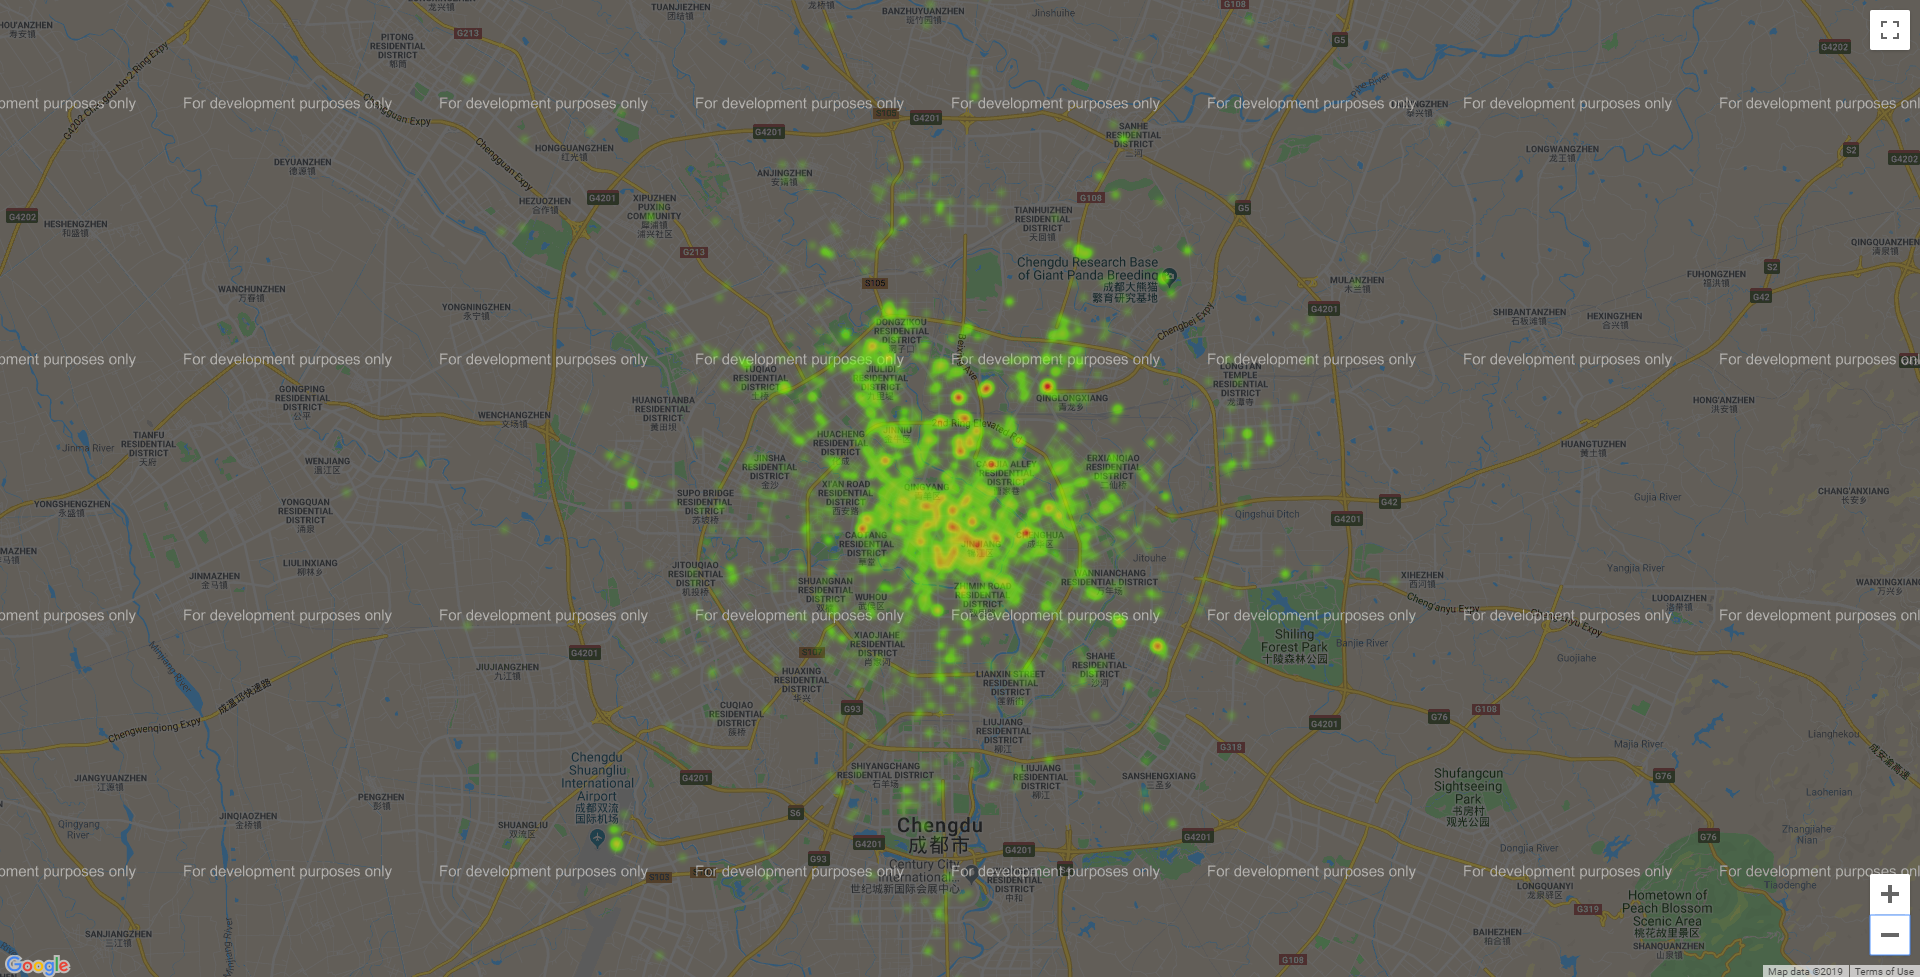
\includegraphics[width=0.9\textwidth]{imgres/9AM_Dropoff.PNG} % second figure itself
    \end{minipage}
    \caption{Heatmaps overlayed on Chengdu City Map for rides starting at 9 A.M. -  $Pickups$ (left) and $\mathit{Dropoffs}$ (right) }
    \label{fig:heatmaps9am}
\end{figure}

% \begin{figure}
%      \centering
%      \begin{subfigure}[b]{0.9\textwidth}
%          \centering
%          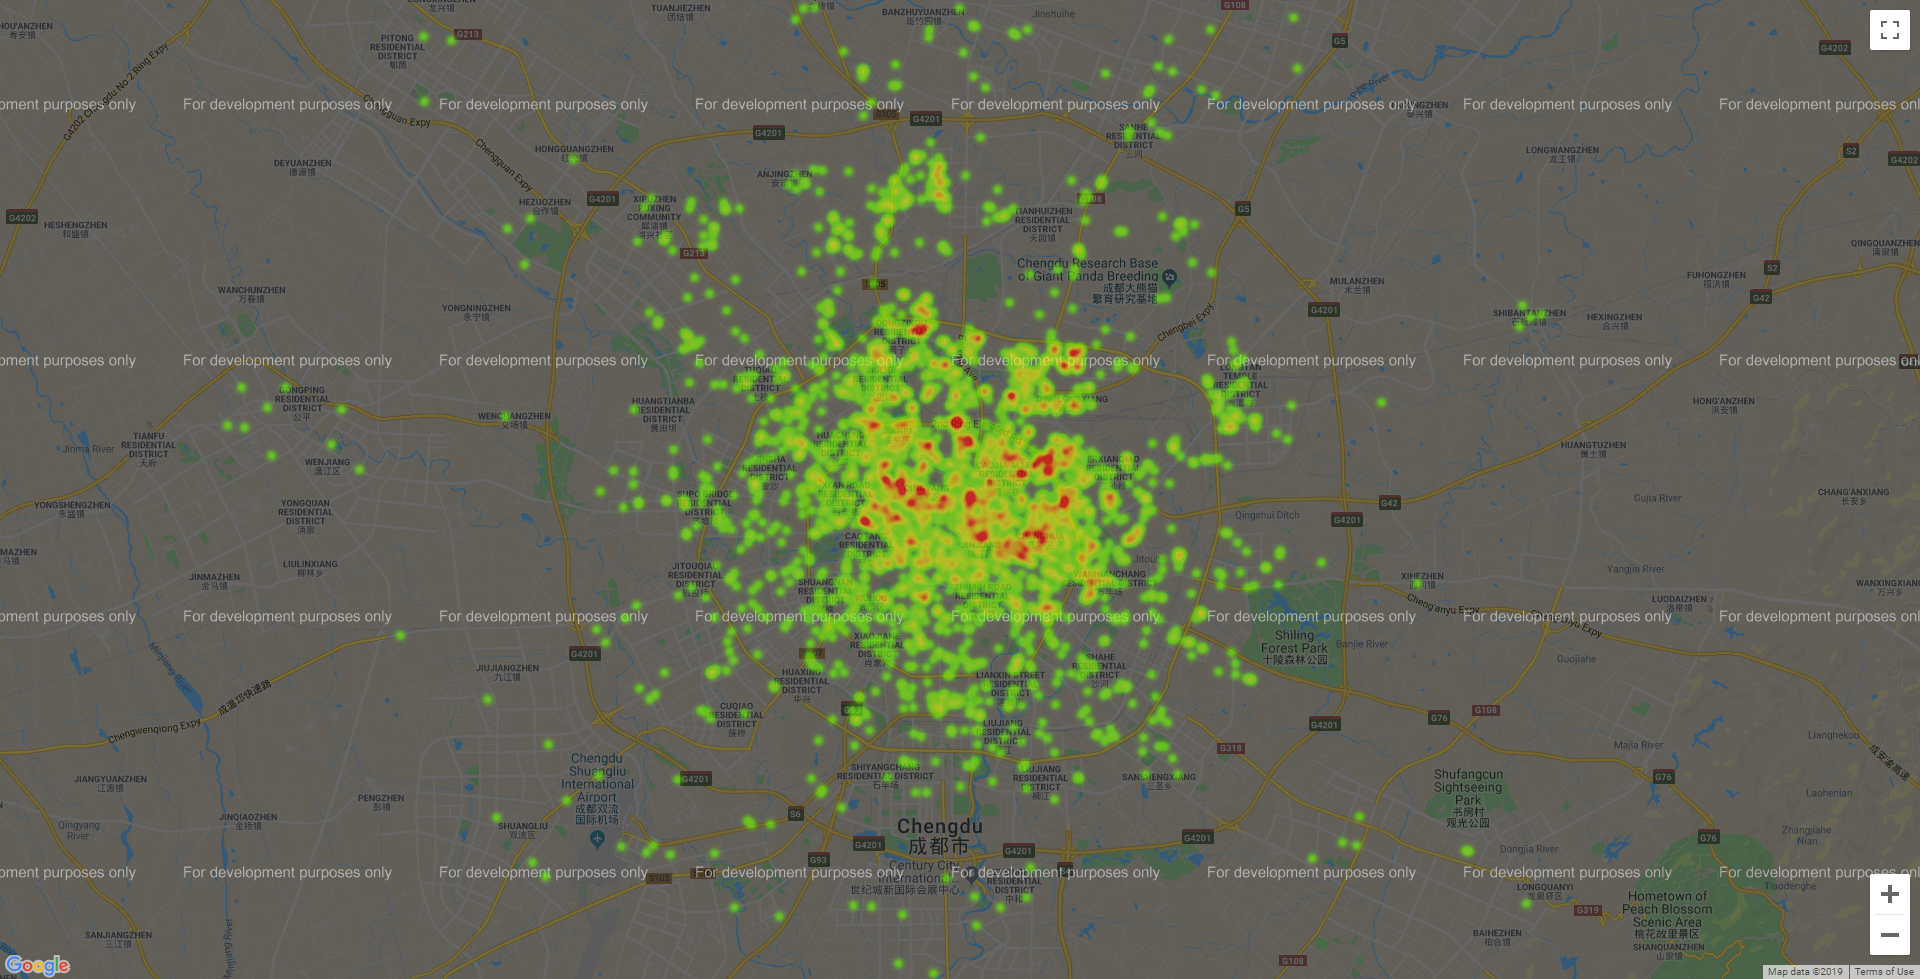
\includegraphics[width=\textwidth]{imgres/9AM_Pickup.PNG}
%          \caption{}
%          \label{fig:9AM}
%      \end{subfigure}
%      \hfill
%      \begin{subfigure}[b]{0.9\textwidth}
%          \centering
%          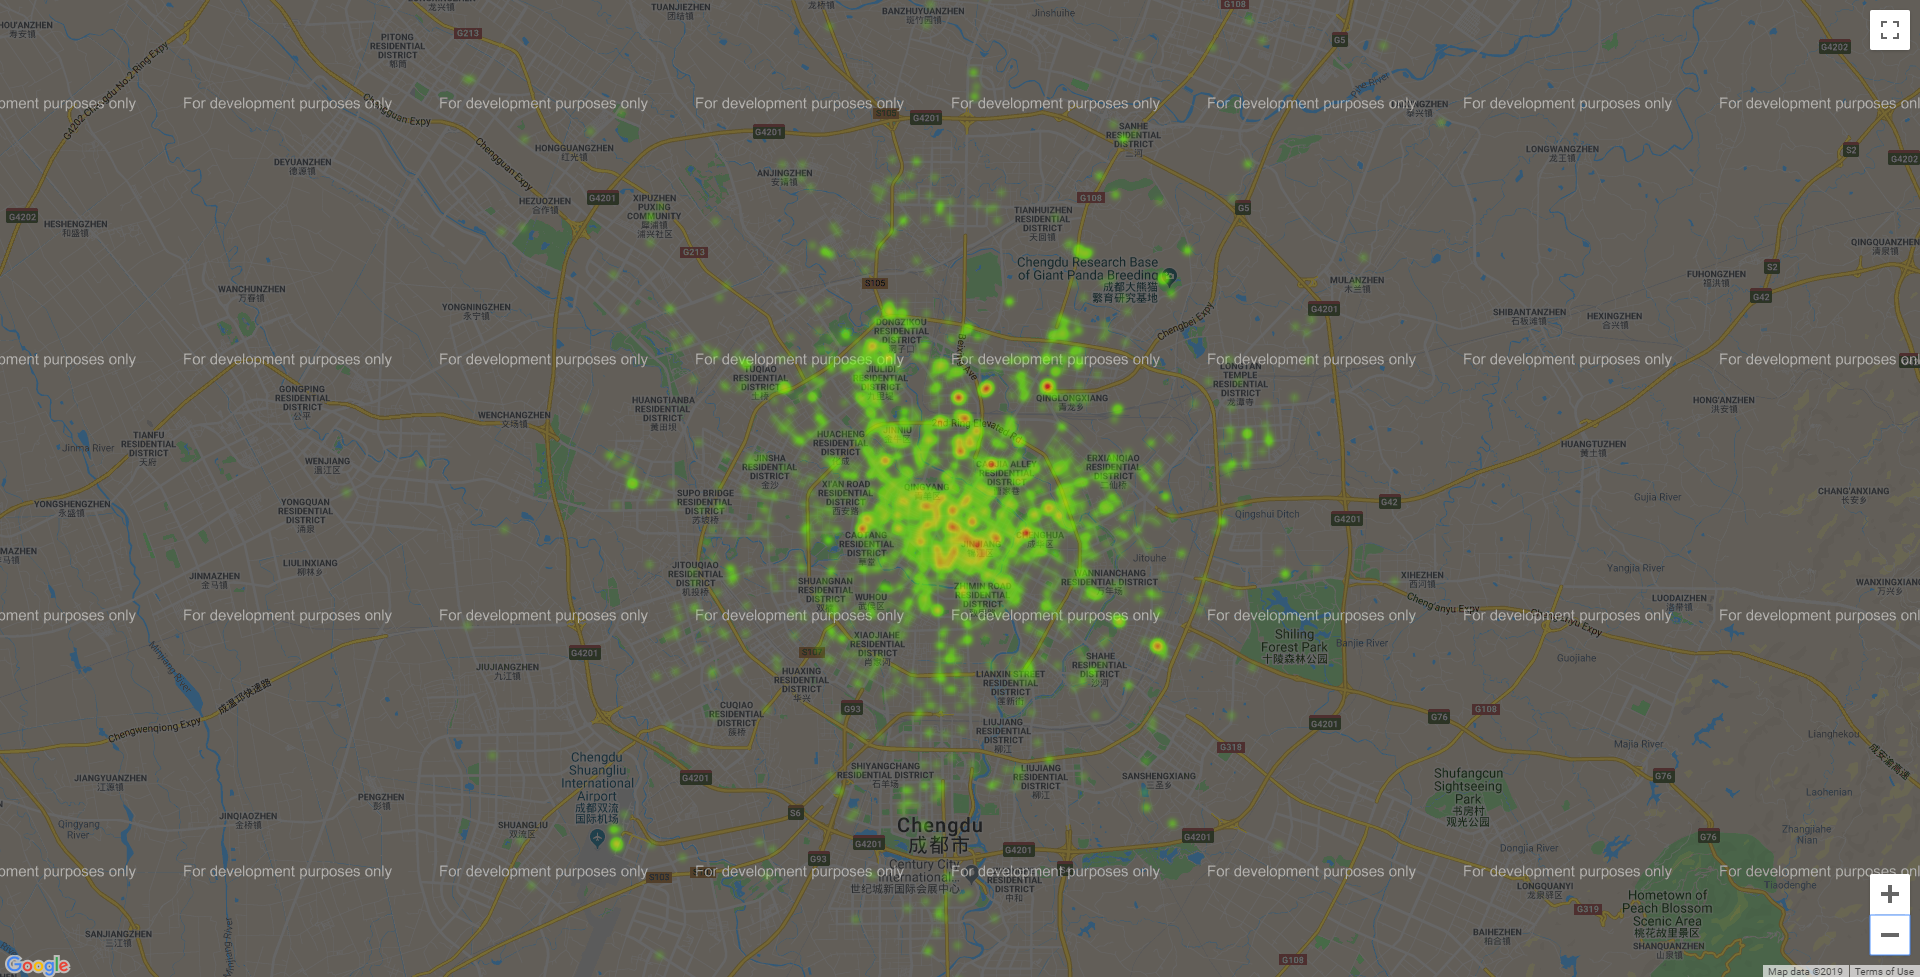
\includegraphics[width=\textwidth]{imgres/9AM_Dropoff.PNG}
%          \caption{}
%          \label{fig:6PM}
%      \end{subfigure}
%      \hfill
%         \caption{Heatmaps overlayed on Chengdu City Map for rides starting at 9 A.M. $(a) Pickups$ and $(b) \mathit{Dropoffs}$ }
%         \label{fig:heatmaps9am}
% \end{figure}

% \begin{figure}
%      \centering
%      \begin{subfigure}[b]{0.9\textwidth}
%          \centering
%          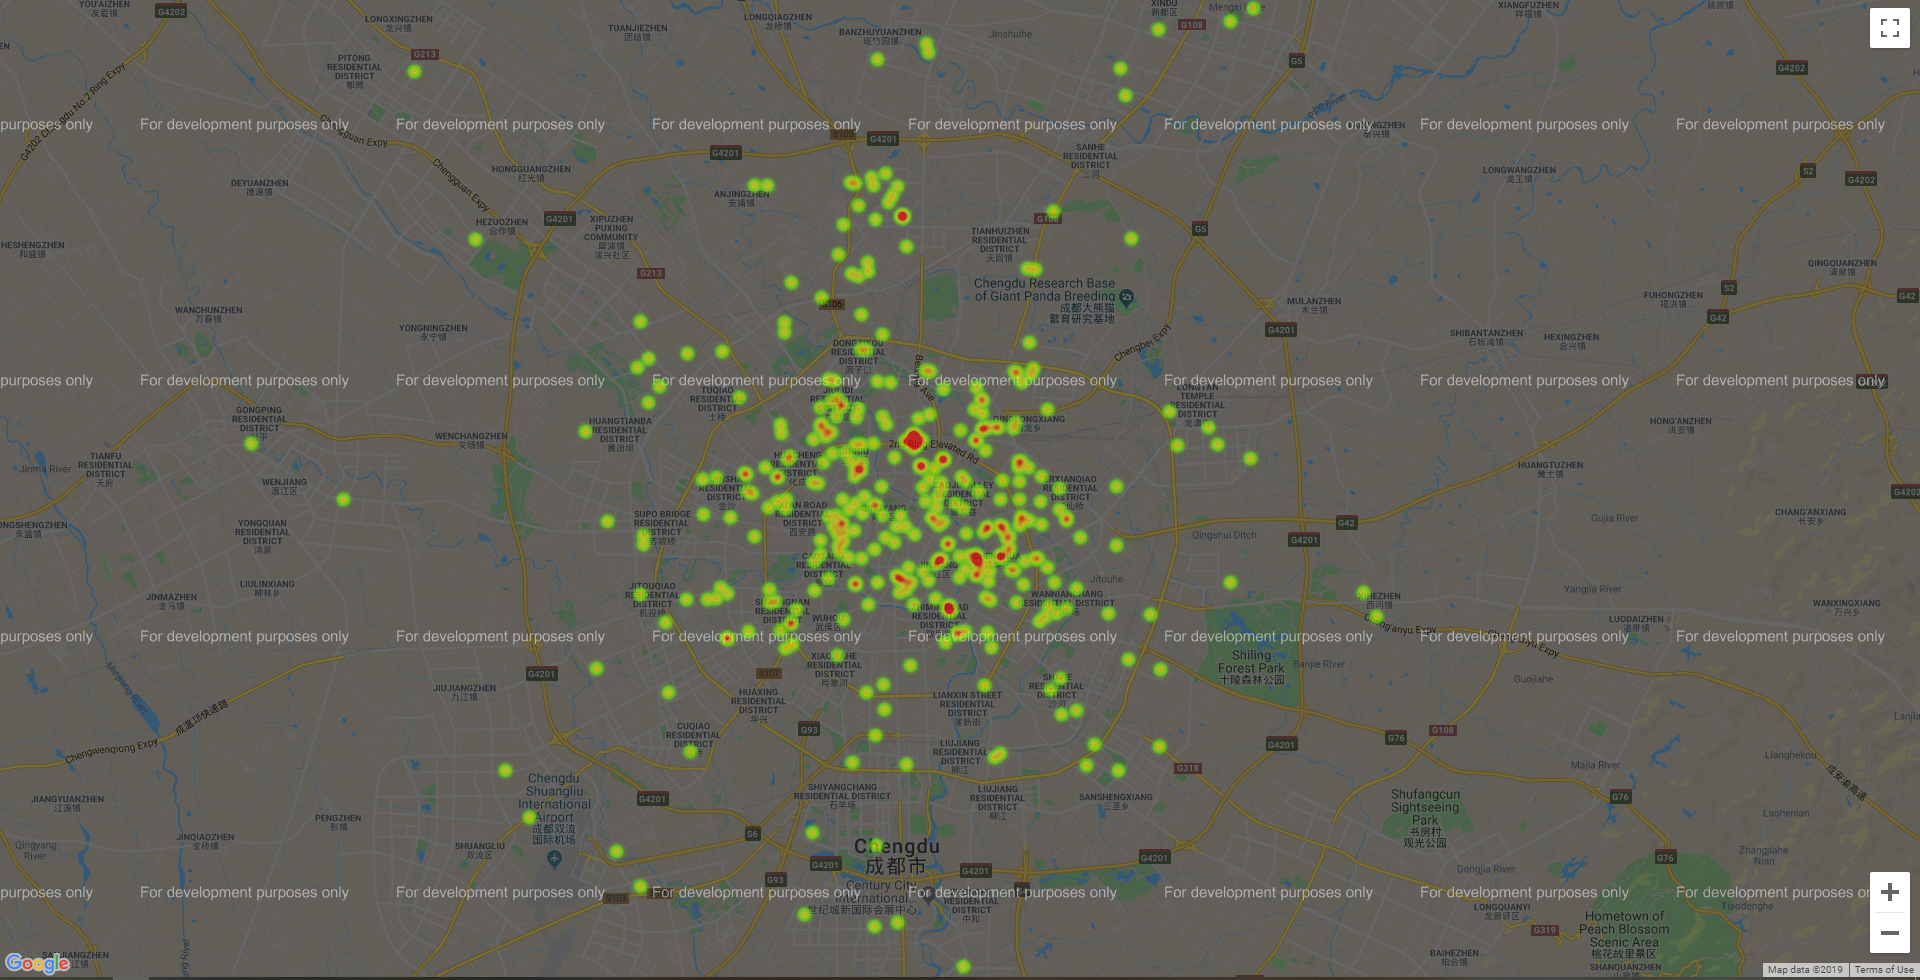
\includegraphics[width=\textwidth]{imgres/6PM_Pickup.PNG}
%          \caption{}
%          \label{fig:9AM}
%      \end{subfigure}
%      \hfill
%      \begin{subfigure}[b]{0.9\textwidth}
%          \centering
%          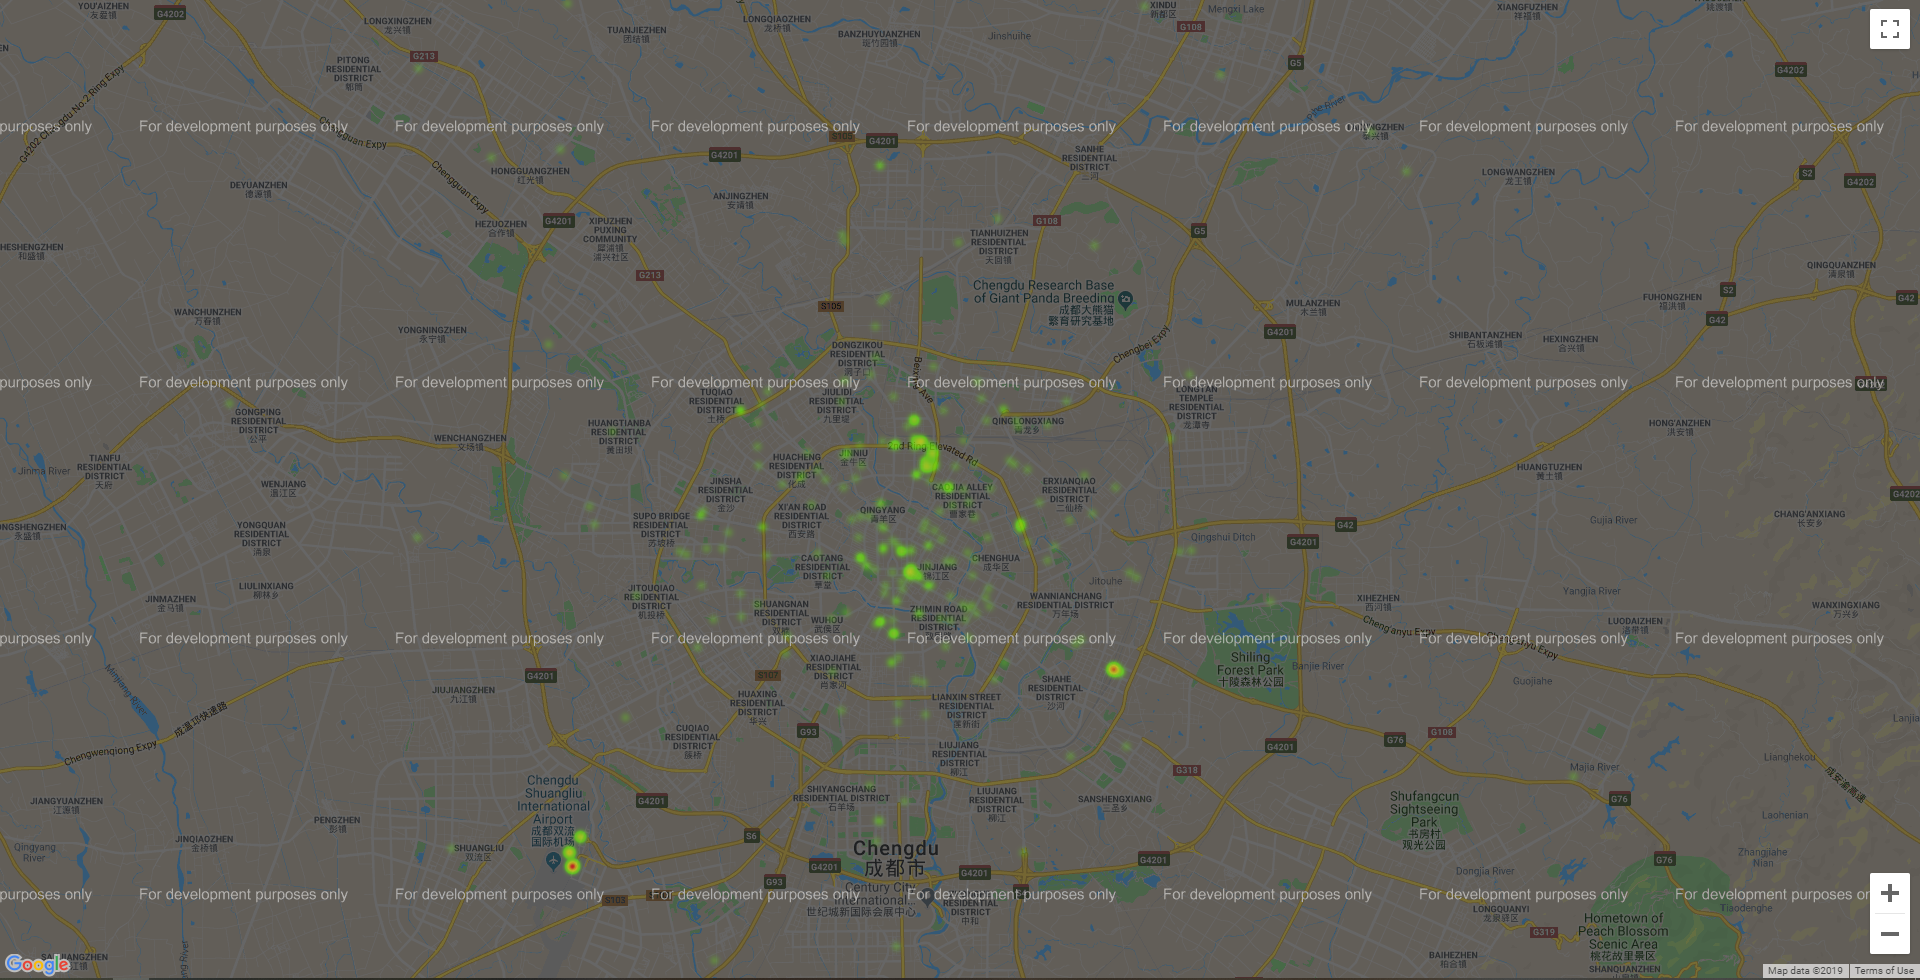
\includegraphics[width=\textwidth]{imgres/6PM_Dropoff.PNG}
%          \caption{}
%          \label{fig:6PM}
%      \end{subfigure}
%      \hfill
%         \caption{Heatmaps overlayed on Chengdu City Map for rides starting at 6 P.M. $(a) Pickups$ and $(b) \mathit{Dropoffs}$ }
%         \label{fig:heatmaps6pm}
% \end{figure}

\begin{figure}
    \centering
    \begin{minipage}{0.45\textwidth}
        \centering
        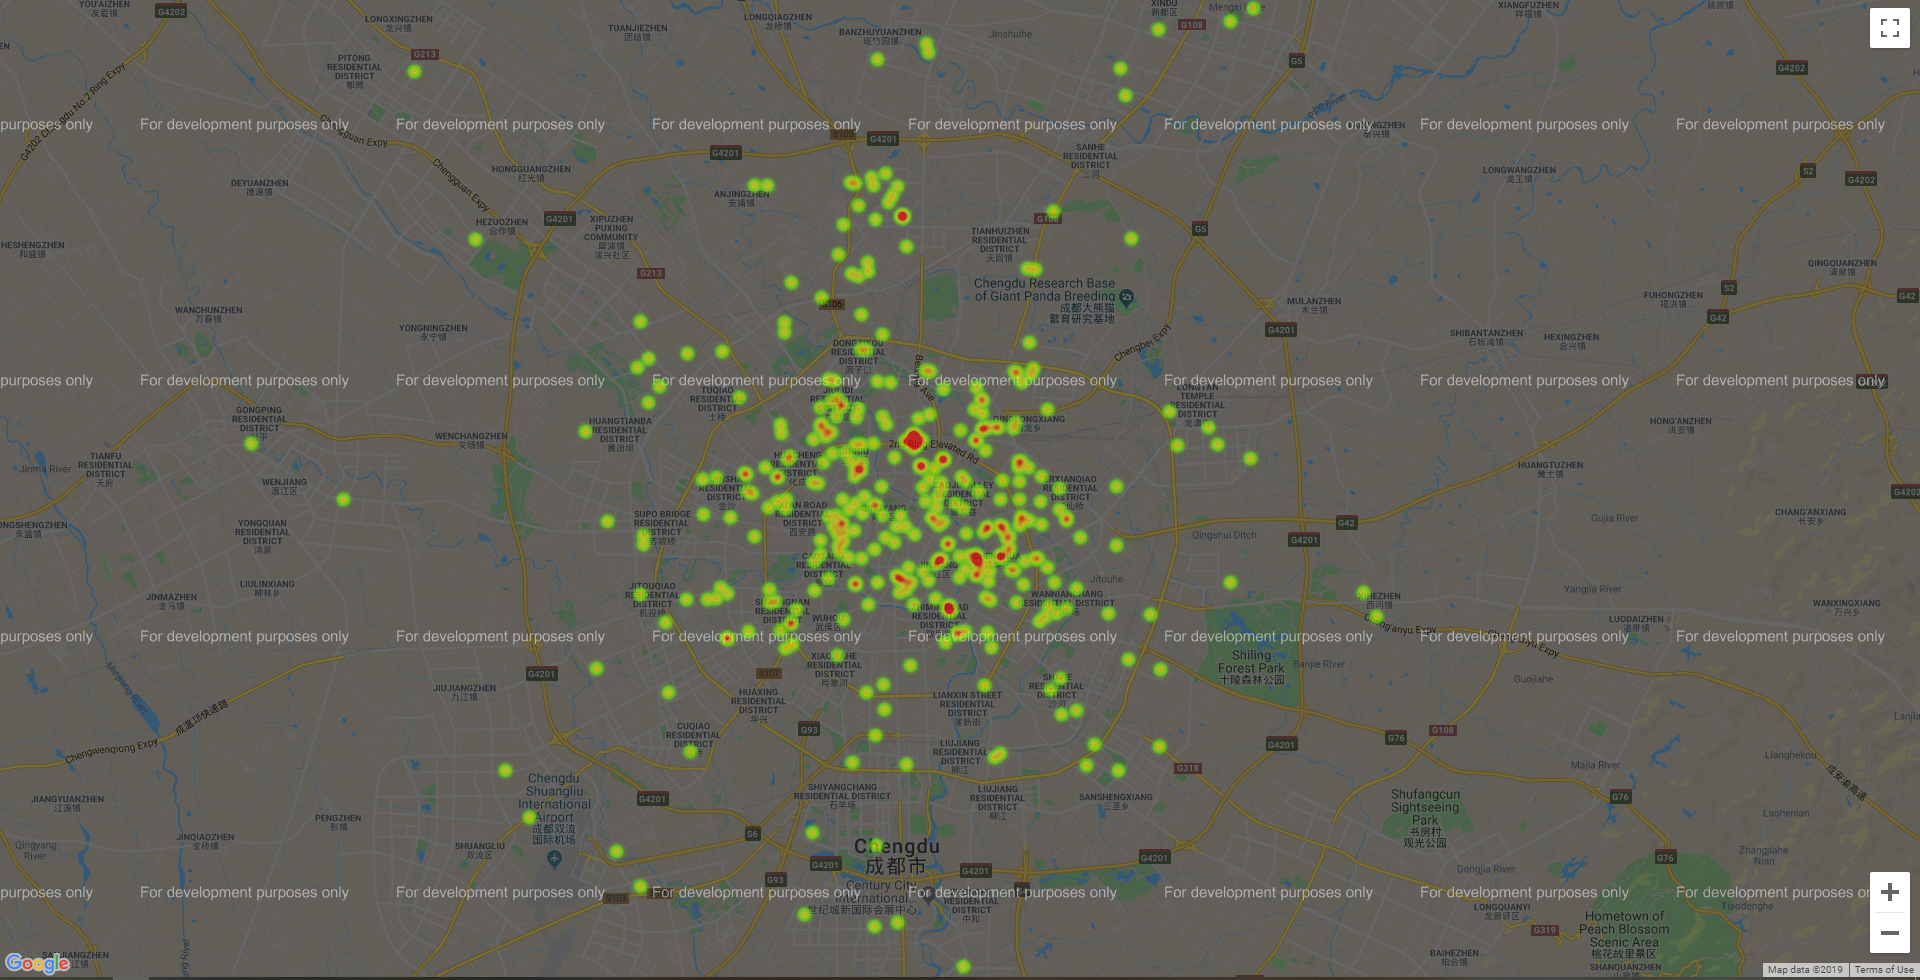
\includegraphics[width=0.9\textwidth]{imgres/6PM_Pickup.PNG} % first figure itself
    \end{minipage}\hfill
    \begin{minipage}{0.45\textwidth}
        \centering
        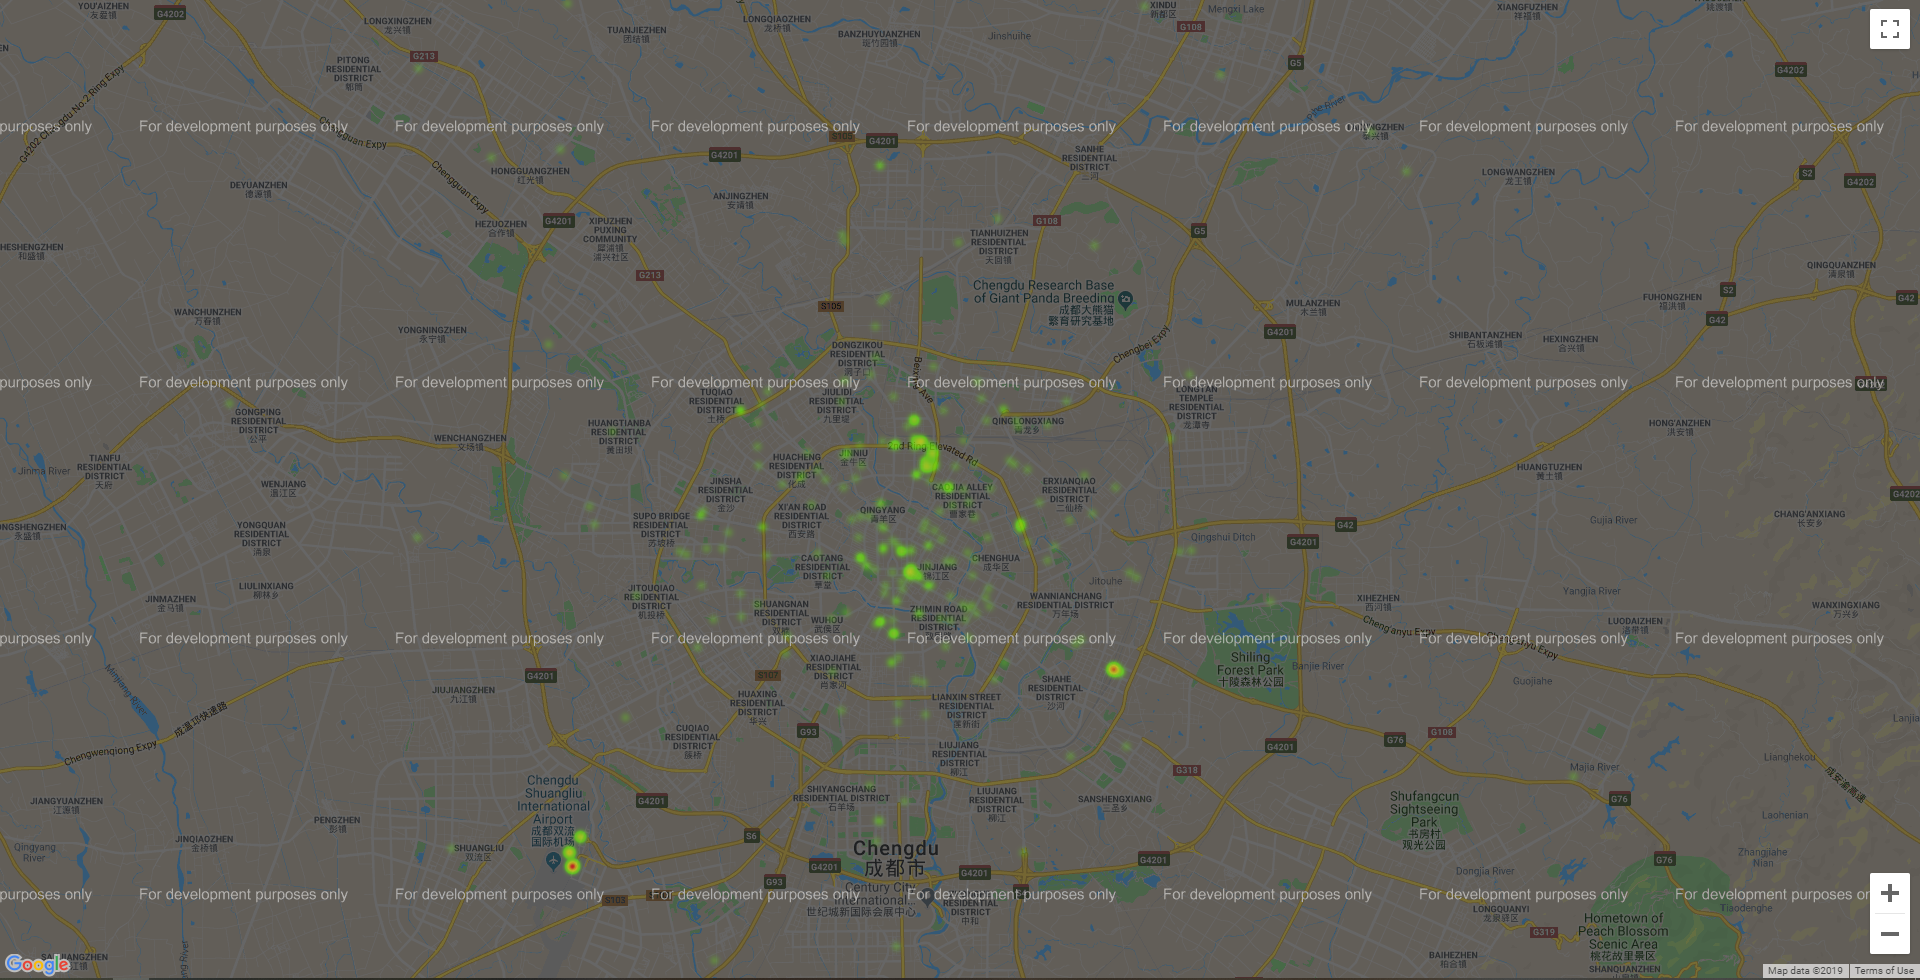
\includegraphics[width=0.9\textwidth]{imgres/6PM_Dropoff.PNG} % second figure itself
    \end{minipage}
    \caption{Heatmaps overlayed on Chengdu City Map for rides starting at 6 P.M. -  $Pickups$ (left) and $\mathit{Dropoffs}$ (right) }
    \label{fig:heatmaps6pm}
\end{figure}

\section{Base Model Development}
\subsection{Problem Formulation}
Our aim is to develop a base model which can explain the performance of the drivers as a function of the available data. The amount of money that a driver makes during a given time period is the best estimator for evaluating the efficiency of driver behavior. However, as the fare data is not available, in this project we use the ratio of the ride time to driver active time, called “Performance Ratio” henceforth, as an approximation of the driver performance. This approximation is based on the assumption that spending more time in a ride will result in raising more money for a specific driver. The remaining parts of this section explain the steps for creating a base model that predicts the Performance Ratio given the driver behavior. 

\subsection{Feature Extraction}
To encode the driver behavior, we aim to extract features that can answer the following questions for each driver:
\begin{enumerate}
\item What are the common locations that the driver drives in? (spatial behavior)
\item During which time periods does the driver take his/her rides? (temporal behavior)
\item What type of rides are allotted to the driver - pool rides, or private rides?
\end{enumerate}

\subsubsection{Spatial Features}
To capture the spatial behavior of the driver, we mesh the entire city with rectangular grids, where the grid-size can be tuned as a hyper-parameter to the model. The percentage of time that a driver spends in each grid is used as a predictive feature. However, since the exact coordinates of the driver at each point during the day are not available, a proxy is required. This is approximated by the number of rides picked up by a driver in a particular grid, as a ratio of the total number of rides picked up by the driver in the whole day. As an example, if a driver picks up 5 rides from zone A, 10 rides from zone B, and 1 ride from zone C, then we use $\frac{5}{16}$, $\frac{10}{16}$, and $\frac{1}{16}$ as the values for the 3 zone features. Assuming that the number of drivers is “n” and that we are using a $10\times10$ grid to cover the entire city, there will be a $n\times100$ feature matrix F, where $F_{i,j}$ is an approximation of the percentage of time that driver “i” spends in the grid j. The goal of this encoding is to capture the spatial preferences of a driver, and to identify  a possible correlation between the driving zone preferences and the Performance Ratio.  
\subsubsection{Temporal Features}
We use temporal features to help us identify if the times that a driver picked up/dropped off passengers have a significant impact on the Performance Ratio. 
For this purpose, we split a day into 4 parts of 6 hours each. We then see how many rides a particular driver picked up or dropped off in that time interval. However, there were more rides during the day, compared to at night. So, splitting into equal parts does not give us similar amounts of data in each time interval. To overcome this problem, we instead calculate percentiles of times. As an example, based on splitting the day into 4 quantiles, we calculate the time splits as 12:00 A.M. - 10:30 A.M., 10:30 A.M. - 2:30 P.M., 2:30 P.M. - 6:30 P.M., and 6:30 P.M. - 12:00 A.M. Splitting into these intervals instead of our original 6 hour intervals gives us an equal amount of data in each of these intervals, on any given day. We then calculate the number of rides picked up by a driver in each time interval, and normalize it by the total number of rides picked up during the day. As an example, if a driver picked up 2 rides between 12:00 A.M - 10:30 A.M, and 4 rides between 6:30 P.M. - 12:00 A.M, the temporal feature values for this driver would be $\frac{1}{3}$, 0, 0, and $\frac{2}{3}$, respectively.


\subsubsection{Space-Time Interaction}
We also consider crosses between spatial features and temporal features. This allows us to identify scenarios such as whether picking up from a certain area during peak hours was positively correlated with a high Performance Ratio. 

\subsubsection{Other Features}
In addition to the spacial and temporal features, we also create variables describing the number of total rides, as well as number of pool rides a driver takes in a day. Formulation of these features is described below:
\newline
\newline
\subsubsubsection{\underline{Pool Rides}:}
Rides where the driver picks up more orders during servicing an ongoing order can be indicative of how active the driver has been in the same period of time as another driver. Since each ride pickup corresponds to a different $order\_id$, we identify potential pool rides whenever the $ride\_start\_time$ for a driver's $order\_id$ preceded the $ride\_stop\_time$ for same driver's previous ride in that day. This variable is used in the model as a fraction of the driver's total number of rides for that day.
\newline
\newline
\subsubsubsection{\underline{Total Number of Rides}:}
This denotes the total number of rides taken by the driver in a given day.

\section{Results of the base model}
We split the data into a training set of 75\%, and test set of 25\%. We first apply a simple linear regression model, with and without regularization (Lasso and Ridge Penalties) to our data. We also try a Random Forest Regressor. Not all features are important, and quite a few spatial features, and most of the cross features have either low feature importances, or have 0 coefficients (in the case of lasso regression). The $\mathit{RMSE}$ on the test set ranges from $\sim0.26$ to $\sim0.60$ using the different models and subset of the features. The lowest $\mathit{RMSE}$ is achieved using Lasso Regression. This is a good start for a base model, but we now plan to add more features, and improve upon some of the na\"ive approximations.

\section{Future Steps}
\begin{itemize}
    \item Improve driver inactive time calculation :
    Our currently defined logic for computing a driver's inactive time is very discrete. We plan to improve upon this by using the following ideology: 
    
    A driver, before starting their first ride of the day or right after ending a ride, would wait for a tolerance ($\tau$) period (in minutes), after which their probability of staying online on the system can be assumed to go down as an exponential distribution. We plan to determine an appropriate value of $\tau$ empirically from the data.
    
    This logic should give a more sophisticated and realistic estimate of the driver's inactive time during a day. A more accurate calculation of this will also directly affect the Performance Ratio.

    \item Formulate more features from existing data:
    Our next step is to use the idle time between two rides as a feature in the model. Hence, instead of na\"ively using the number of rides picked up from a particular zone as a proxy of the spatial feature, we can be more intelligent by splitting the idle time of a driver between the last drop off and next pick up. This will allow us to better approximate the spatial features.
    \item Go from a linear model to non-linear models:
    So far, we have have used linear models. An advantage of linear models is that they make explanations of feature importances much easier. However, we plan to go into the realm of non-linear models, and try different non-linear models for this data as well.
    \item Use techniques like Inverse Reinforcement Learning: We could potentially learn a policy from the general trajectory data. The aim is to try an extract a policy that is implied by the trajectory representation, and inverse reinforcement learning has been successful in the past in order to achieve this.
\end{itemize}


\section{Acknowledgements}
We are extremely thankful to our mentors, Professor Vineet Goyal (IEOR, Columbia University) and Zhiwei (Tony) Qin (DiDi Labs/ AI Labs). Their suggestions during our weekly meetings have been very useful for deciding our modeling approach and feature selection, and are invaluable for our project. We would also like to thank Sining Chen (DSI, Columbia University) for providing us with a guideline and advising us on the best practices for a report. 


\section{References} 
\begin{enumerate}
    \item \href{https://outreach.didichuxing.com/research/opendata/en/}{DiDi GAIA Open Data Initiative}
    
    \item \href{https://github.com/rmahajan14/capstone_didi}{Project Github Repository}
    
    \item Liu, L., Andris, C., Ratti, C., Nov. 2010. Uncovering cabdrivers' behavior patterns from their digital traces. Computers, Environment and Urban Systems 34 (6), 541-548.
    
    \item Li, B., Zhang, D., Sun, L., Chen, C., Li, S., Qi, G., Yang, Q., Mar. 2011. Hunting or waiting? Discovering passenger finding strategies from a large-scale real-world taxi dataset. In: 2011 IEEE International Conference on Pervasive Computing and Communications Workshops (PERCOM Workshops). pp. 63-68.
    
    \item Shou, Z., Di, X., Ye, J., Zhu, H., Zhang, H., Hampshire, R.,. Oct. 2019. Optimal Passenger-Seeking Policies on E-hailing Platforms Using Markov Decision Process and Imitation Learning. arXiv:1905.09906
    
    \item Holler, B., Qin, Z., Tang, X., Jiao, Y., Jin, T., Singh S., Wang C., Ye, J. 2018. Deep Q-Learning Approaches to Dynamic Multi-Driver Dispatching and Repositioning. 32nd Conference on Neural Information Processing Systems (NIPS 2018), Montréal, Canada.
    
     \item Xiaocheng Tang,Zhiwei (Tony) Qin, Fan Zhang
AI Labs, Didi Chuxing
    
\end{enumerate}


\section{Attribution}
\begin{enumerate}[label*=\arabic*.]
    \item Project Introduction: Ashwin, Ridhi
    \item Literature Review: Foad
    \item Initial Data Exploration/Visualization
    \begin{enumerate}[label*=\arabic*.]
        \item Dataset Description: Akshat, Ashwin
        \item Data Challenges: Ridhi, Akshat
        \item Data Visualization: Akshat, Ashwin
    \end{enumerate}
    \item Base Model Development
    \begin{enumerate}[label*=\arabic*.]
        \item Problem Formulation: Nima, Foad
        \item Feature Extraction: Nima, Foad
        \begin{enumerate}[label*=\arabic*.]
            \item Spatial Features: Nima, Ridhi
            \item Temporal Features: Akshat, Ridhi
            \item Space-Time Interaction: Ridhi
            \item Other Features: Akshat
        \end{enumerate}
    \end{enumerate}
    \item Results of the base model: Nima, Ridhi
    \item Future Steps: Ridhi, Akshat
\end{enumerate}

% 1  \newline
% 2  \newline
% 3   \newline
% 3.1  \newline
% 3.2  \newline
% 3.3  \newline
% 4   \newline
% 4.1  \newline
% 4.2  \newline
% 4.2.1  \newline
% 4.2.2  \newline
% 4.2.3  \newline
% 4.2.4  \newline
% 5  \newline
% 6  \newline

\end{document}
